\documentclass[letterpaper,10pt]{article}

\usepackage{color}
\usepackage{tikz}
\usepackage{caption}

\setlength{\headheight}{0in}
\setlength{\marginparsep}{0in}
\setlength{\footskip}{0in}
\setlength{\headsep}{0in}
\setlength{\marginparwidth}{0in}
\setlength{\marginparpush}{0in}
\setlength{\voffset}{0in}
\setlength{\hoffset}{-1in}
\setlength{\voffset}{-1in}
\setlength{\oddsidemargin}{0.75in}
\setlength{\evensidemargin}{0.75in}
\setlength{\topmargin}{0.75in}
\setlength{\textheight}{9.5in}
\setlength{\textwidth}{7in}
\setlength{\parindent}{0in}
\setlength{\parskip}{10pt} %change this to match font size

\pagestyle{empty}
\definecolor{gray}{gray}{0.75}
\usetikzlibrary{shapes,arrows,calc}

% define block styles
\tikzstyle{line} = [draw, -latex']
\tikzstyle{block} = [draw, rectangle, text centered, minimum height=2em]
\tikzstyle{mlblock} = [draw, rectangle, text width=10em, text centered, minimum height=2em]
\tikzstyle{decision} = [draw, diamond, text width=4.5em, text centered, node distance=3cm, inner sep=0pt]
\tikzstyle{cloud} = [draw, rectangle, text centered, rounded corners, minimum height=2em]

\begin{document}
    Albert Chang and Nipun Chopra\\
    CSE-380 A6\\
    University at Buffalo\\
    Dr. Kris Schindler\\
    March 22, 2011\\
    \textit{Lab 6 Documentation}

    The objective of Lab 6 was to learn how to use the 32-bit timer. A curses-like
    environment is output to the terminal, with an asterisk bouncing back and
    forth. With the keyboard, the user can adjust the speed and direction of
    the asterisk. All of this is accomplished with interrupts.

    The following routines were imported through the \textit{library.s} file:
    \textit{uart\_init}, \textit{output\_character}, \textit{read\_character},
    and \textit{output\_string}. Figs. \ref{flo:uart_init},
    \ref{flo:io_char}, and \ref{flo:output_string} are their respective
    flowcharts for each routine.

    \begin{figure}[h]
        \begin{center}
    \begin{tikzpicture}[node distance = 3cm, auto]
        \node[cloud] (origin) {Start};
        \node[block, below of=origin, node distance=1.5cm] (enable) {Write 0x5 to PINSEL0 to enable UART0};
        \node[mlblock, below of=enable] (init) {Configure U0LCR:\\%
                                                8-bit word length\\%
                                                1 stop bit\\%
                                                no parity\\%
                                                disable break control\\%
                                                enable access latch};
        \node[block, below of=init] (baud) {Set baud rate to 9600};
        \node[mlblock, below of=baud] (conf) {Configure U0LCR:\\%
                                                8-bit word length\\%
                                                1 stop bit\\%
                                                no parity\\%
                                                disable break control\\%
                                                disable latch access};
        \node[cloud, below of=conf] (stop) {Stop};
        \path[line] (origin) -- (enable);
        \path[line] (enable) -- (init);
        \path[line] (init) -- (baud);
        \path[line] (baud) -- (conf);
        \path[line] (conf) -- (stop);
    \end{tikzpicture}
\end{center}

        \caption{Flowchart of \textit{uart\_init} routine.}
        \label{flo:uart_init}
    \end{figure}

    \begin{figure}[h]
        \begin{minipage}{0.5\linewidth}
            \begin{center}
    \begin{tikzpicture}[node distance = 1.5cm, auto]
        \node[cloud] (origin) {Start};
        \node[decision, below of=origin] (test) {Test THRE in status register};
        \node[block, below of=test, node distance = 3.5cm] (store) {Store byte in transmit register};
        \node[cloud, below of=store] (stop) {Stop};
        \path[line] (origin) -- (test);
        \path[line] (test) -- node [near start] {1} (store);
        \path[line] (test) -| node [near start] {0} +(3,2.25) -- +(0,2.25);
        \path[line] (store) -- (stop);
    \end{tikzpicture}
\end{center}

        \end{minipage}%
        \begin{minipage}{0.5\linewidth}
            \begin{center}
    \begin{tikzpicture}[node distance = 1.5cm, auto]
        \node[cloud] (origin) {Start};
        \node[decision, below of=origin] (test) {Test RDR in status register};
        \node[block, below of=test, node distance = 3.5cm] (read) {Read byte from receive register};
        \node[cloud, below of=read] (stop) {Stop};
        \path[line] (origin) -- (test);
        \path[line] (test) -- node [near start] {1} (read);
        \path[line] (test) -| node [near start] {0} +(3,2) -- +(0,2);
        \path[line] (read) -- (stop);
    \end{tikzpicture}
\end{center}

        \end{minipage}
        \caption{Flowcharts of \textit{output\_character} (left) and \textit{read\_character} (right) routines.}
        \label{flo:io_char}
    \end{figure}

    \begin{figure}[h]
        \begin{center}
    \begin{tikzpicture}[node distance = 1.5cm, auto]
        \node[cloud] (origin) {Start};
        \node[block, below of=origin] (read) {Load byte from memory};
        \node[decision, below of=read] (null) {Is it the null character?};
        \node[cloud, below of=null,node distance=3cm] (stop) {Stop};
        \path[line] (origin) -- (read);
        \path[line] (read) -- (null);
        \path[line] (null) -| node [near start] {no} +(3,3) -- (read);
        \path[line] (null) -- node [near start] {yes} (stop);
    \end{tikzpicture}
\end{center}

        \caption{Flowchart of \textit{output\_string} routine.}
        \label{flo:output_string}
    \end{figure}

    \clearpage

    Just as with the previous lab, the main routine, \textit{lab6}, doesn't do
    much besides call upon the initialization routines, \textit{uart\_init} and
    \textit{interrupt\_init}. Afterwards it sets up the initial speed of the
    asterisk, provides the initial output, and starts the timer. The output is
    only changed when something has changed, instead of every cycle. Changes
    are only made when the timer count register matches the match register.

    \begin{minipage}{\linewidth}
        \begin{center}
    \begin{tikzpicture}[node distance = 1.5cm, auto]
        \node[cloud] (origin) {Start};
        \node[block, below of=origin] (uart) {UART setup};
        \node[block, below of=uart] (ui1) {Get user input 1};
        \node[block, below of=ui1] (val1) {Convert to integer};
        \node[decision, below of=val1] (chck1) {Is it a valid input?};
        \node[block, below of=chck1, node distance=3cm] (ui2) {Get user input 2};
        \node[block, below of=ui2] (val2) {Convert to integer};
        \node[decision, below of=val2] (chck2) {Is it a valid input?};
        \node[block, below of=chck2, node distance=3cm] (format) {Format Output};
        \node[block, below of=format] (mod) {Perform modulo};
        \node[block, below of=mod] (ans) {Convert answer to string};
        \node[block, below of=ans] (output) {Output answer};
        \node[cloud, below of=output] (stop) {Stop};
        \path[line] (origin) -- (uart);
        \path[line] (uart) -- (ui1);
        \path[line] (ui1) -- (val1);
        \path[line] (val1) -- (chck1);
        \path[line] (chck1) -- node [near start] {yes} (ui2);
        \path[line] (chck1) -| node [near start] {no} +(3,4.5) -- (ui1);
        \path[line] (ui2) -- (val2);
        \path[line] (val2) -- (chck2);
        \path[line] (chck2) -- node [near start] {yes} (format);
        \path[line] (chck2) -| node [near start] {no} +(3,4.5) -- (ui2);
        \path[line] (format) -- (mod);
        \path[line] (mod) -- (ans);
        \path[line] (ans) -- (output);
        \path[line] (output) -- (stop);
    \end{tikzpicture}
\end{center}

        \captionof{figure}{Flowchart of \textit{lab6} routine.}
        \label{flo:main}
    \end{minipage}

    The \textit{interrupt\_init} routine is similar to the previous lab's,
    except instead of enabling and configuring the external interrupt, it
    enables and configures timer interrupt.

    \begin{minipage}{\linewidth}
        \begin{center}
    \begin{tikzpicture}[node distance=1.5cm, auto]
        \node[cloud] (origin) {Start};
        \node[block, below of=origin] (fiq) {Classify as FIQs};
        \node[block, below of=fiq] (enable) {Enable UART0, TIMER0, TIMER1, and EINT1 interrupts};
        \node[block, below of=enable] (uart) {UART0 interrupt on RX};
        \node[block, below of=uart] (timers) {Setup TIMER interrupts};
        \node[block, below of=timers] (eint) {EINT1 interrupts on edge};
        \node[block, below of=eint] (cpsr) {Enable fast interrupts on CPSR};
        \node[cloud, below of=cpsr] (stop) {Stop};
        \path[line] (origin) -- (fiq);
        \path[line] (fiq) -- (enable);
        \path[line] (enable) -- (uart);
        \path[line] (uart) -- (timers);
        \path[line] (timers) -- (eint);
        \path[line] (eint) -- (cpsr);
        \path[line] (cpsr) -- (stop);
    \end{tikzpicture}
\end{center}

        \captionof{figure}{Flowchart of \textit{interrupt\_init} routine.}
        \label{flo:interrupt_init}
    \end{minipage}

    Again, the bulk of the program is handled by the fast interrupt handler,
    \textit{FIQ\_Handler}. Depending on which kind of interrupt it is, it takes
    the appropriate action.

    \begin{minipage}{\linewidth}
        \begin{center}
    \begin{tikzpicture}[node distance=1.5cm, auto]
        \node[cloud] (origin) {Start};
        \node[decision, below of=origin] (timer) {Was the interrupt caused by the timer?};
        \node[block, below of=timer, node distance=3cm] (clear) {Clear interrupt};
        \node[block, below of=clear] (fixed) {Clear terminal and output prompt and top of box};
        \node[block, below of=fixed] (get) {Get position and direction};
        \node[block, below of=get] (updatep) {Update position and change direction if necessary};
        \node[block, below of=updatep] (updatet) {Update terminal output};
        \node[block, below of=updatet] (save) {Save positition and direction};
        \node[block, below of=save] (reset) {Reset TCR and re-enable clock};
        \node[decision, below of=reset] (uart) {Was the interrupt caused by UART?};
        \node[block, below of=uart, node distance=3cm] (input) {Read input};
        \node[block, below of=input] (set) {Adjust speed and direction based on input};
        \node[cloud, below of=set] (stop) {Stop};
        \path[line] (origin) -- (timer);
        \path[line] (timer) -- node [near start] {yes} (clear);
        \path[line] (clear) -- (fixed);
        \path[line] (fixed) -- (get);
        \path[line] (get) -- (updatep);
        \path[line] (updatep) -- (updatet);
        \path[line] (updatet) -- (save);
        \path[line] (save) -- (reset);
        \path[line] (reset) -- (uart);
        \path[line] (uart) -- node [near start] {yes} (input);
        \path[line] (input) -- (set);
        \path[line] (set) -- (stop);
        \path[line] (timer) -| node [near start] {no} +(6,-21) -- (stop);
        \draw (uart) -- node [near start] {no} +(6,0);
    \end{tikzpicture}
\end{center}

        \captionof{figure}{Flowchart of \textit{FIQ\_Handler} routine.}
        \label{flo:fiq_handler}
    \end{minipage}

    There wasn't really a clear distribution of labor. It was all programmed in
    one lab session via pair programming.

\end{document}
